\section{Άσκηση 3}

\subsection{Υποερώτημα α}

Επειδή $b \ll a$ μπορούμε να θεωρήσουμε ότι το μαγνητικό πεδίο του βρόγχου
$C_2$ προσεγγίζεται από ένα μαγνητικό δίπολο $\vec{m} = I_2\pi b^2
\hat{\mathbf{z}}$.

\begin{figure*}
  \centering
  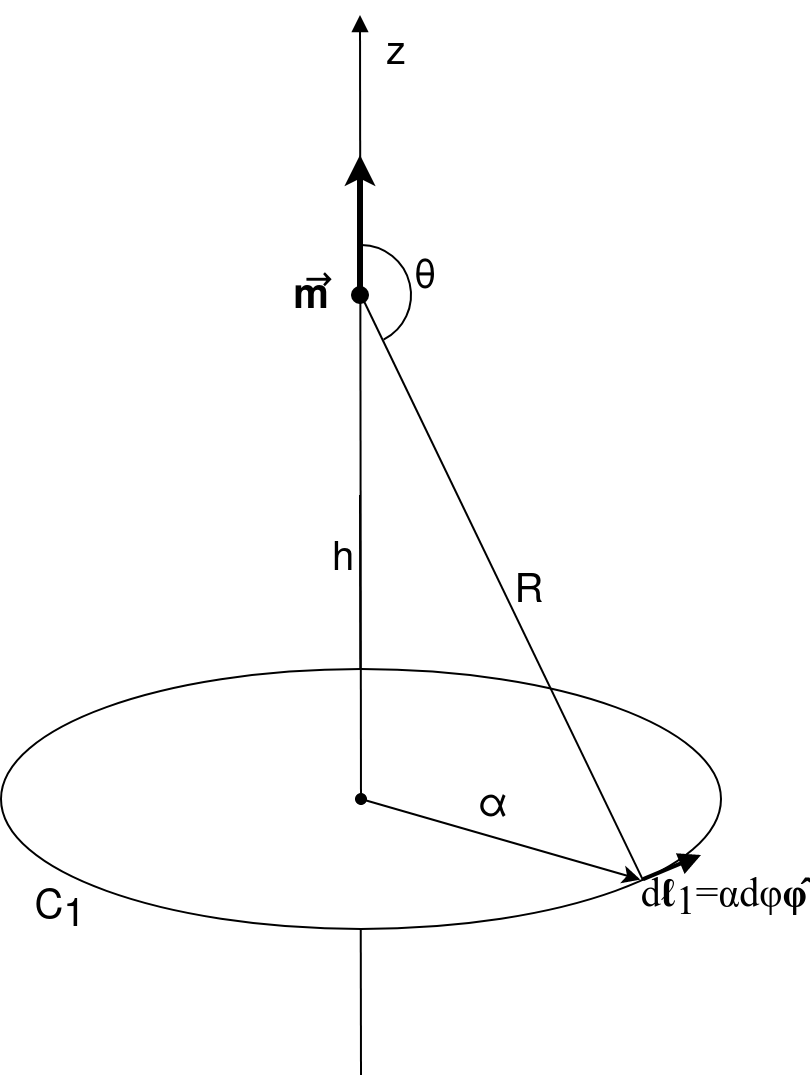
\includegraphics[scale=0.25]{figures/figure_dipole.png}
  \caption{Η διάταξη προσέγγισης.}
  \label{fig:problem-5}
\end{figure*}

Το διανυσματικό δυναμικό $Α_1$ λόγω του μαγνητικού διπόλου δίνεται από 


% \begin{equation} \label{eq1}
% \begin{split}
%   1: & 0 \leq r \leq b \\
%   2: & b \leq r \leq a \\
%   3: & a \leq r
% \end{split}
% \end{equation}

% Αρχικά ορίζουμε τρεις περιοχές του χώρου:
% 
% \begin{equation} \label{eq1}
% \begin{split}
%   1: & 0 \leq r \leq b \\
%   2: & b \leq r \leq a \\
%   3: & a \leq r
% \end{split}
% \end{equation}
% 
% \subsection{Εύρεση δυναμικού}
% 
% Σε όλες τις περιοχές υπάρχει ή κενό ή αφόρτιστο διηλεκτρικό, συνεπώς ισχύει η
% εξίσωση Poisson για το δυναμικό:
% 
% \[ \nabla^{2}\Phi = 0 \]
% 
% Λόγω της συμμετρίας της διάταξης το δυναμικό σε κάθε περιοχή $i$ θα είναι της
% μορφής $\Phi_{i} = \Phi_{i}(r)$. Συνεπώς, λύνοντας την διαφορική εξίσωση έχουμε
% 
% 
% \begin{equation} \label{eq1}
% \begin{split}
%            & \nabla^{2}\Phi_{i} = 0 \\
%   \implies & \frac{1}{r^{2}}\frac{\partial}{\partial r}(r^{2}\frac{\partial \Phi_{i}}{\partial r}) = 0 \\
%   \implies & r^{2}\frac{\partial \Phi_{i}}{\partial r} = A_{i} \\
%   \implies & \frac{\partial \Phi_{i}}{\partial r} = \frac{A_{i}}{r^{2}} \\
%   \implies & \Phi_{i} = B_{i} - \frac{A_{i}}{r}
% \end{split}
% \end{equation}
% 
% Στην περιοχή 1 παρατηρούμε ότι η προφανής λύση $\Phi_{1}(r) = V_{b}$ ικανοποιεί
% την διαφορική εξίσωση και την συνοριακή συνθήκη $\Phi_{1}(b) = V_{b}$. Από
% το θεώρημα μοναδικότητας ξέρουμε ότι αυτή είναι και η σωστή λύση. Συπεπώς
% $A_{1} = 0$ και $B_{1} = 0$.
% 
% Στην περιοχή 2 μέσω των δύο συνοριακών συνθηκών $\Phi_{2}(b) = V_{b}$ και
% $\Phi_{2}(a) = V_{a}$ καταλήγουμε σε ένα σύστημα δύο εξισώσεων.
% 
% \begin{equation} \label{eq1}
% \begin{split}
%   B_{2} - \frac{A_{2}}{a} & = V_{a} \\
%   B_{2} - \frac{A_{2}}{b} & = V_{b}
% \end{split}
% \end{equation}
% 
% Λύνοντας το σύστημα και αντικαθιστόντας στη (2) παίρνουμε το δυναμικό στην περιοχή 2.
% 
% \[ \Phi_{2}(r) = \frac{bV_{b} - aV_{a}}{b - a} - \frac{V_{b} - V_{a}}{b-a}\cdot\frac{ab}{r} \]
% 
% Τέλος, στην περιοχή 3 από τη συνθήκη στο άπειρο προκύπτει ότι
% 
% \[ \Phi_{3}(r\to\infty) = 0 \implies B_{3} = 0 \]
% 
% Και από τη συνοριακή συνθήκη στο $r = a$ έχουμε
% 
% \begin{equation} \label{eq1}
% \begin{split}
%      \Phi_{3}(a) & = -\frac{A_{3}}{a} = V_{a} \\
%   \implies A_{3} & = -aV_{a}
% \end{split}
% \end{equation}
% 
% Άρα τελικά το δυναμικό σε όλο τον χώρο είναι
% 
% \[ \Phi(r) = \left\{
%               \begin{array}{lr}
%                 V_{b}                                                                         & 0 \leq r \leq b \\
%                 \frac{bV_{b} - aV_{a}}{b - a} - \frac{V_{b} - V_{a}}{b-a}\cdot\frac{ab}{r}    & b \leq r \leq a \\
%                 V_{a}\frac{a}{r}                                                              & a \leq r
%               \end{array}
%             \right.
% \]
% 
% \subsection{Εύρεση ηλεκτρικού πεδίου}
% 
% Το ηλεκτρικό πεδίο βρίσκεται από τη σχέση $\textbf{E} = -\nabla \Phi$ σε κάθε
% περιοχή του χώρου. Συνεπώς το ηλεκτρικό πεδίο θα είναι:
% 
% \[ \textbf{E}(r) = \left\{
%               \begin{array}{lr}
%                 0\hat{\mathbf{r}}                                                & 0 \leq r \leq b \\
%                 -\frac{V_{b} - V_{a}}{b-a}\cdot\frac{ab}{r^{2}}\hat{\mathbf{r}}  & b \leq r \leq a \\
%                 V_{a}\frac{a}{r^{2}}\hat{\mathbf{r}}                             & a \leq r
%               \end{array}
%             \right.
% \]
% 
% \subsection{Επιφανειακές πυκνότητες φορτίου}
% 
% Στην επιφάνεια $r=b$ ισχύει η οριακή συνθήκη $\sigma(r=b) =
% \hat{\mathbf{r}}\cdot(\textbf{D}(b_{+}) - \textbf{D}(b_{-}))$. Αντικαθιστώντας έχουμε
% 
% \begin{equation} \label{eq1}
% \begin{split}
%   \sigma(r=b) & = D_{r}(b_{+}) - D_{r}(b_{-}) \\
%               & = -\epsilon_{a}\frac{V_{b} - V_{a}}{b-a}\cdot\frac{b}{a}
% \end{split}
% \end{equation}
% 
% Στην επιφάνεια $r=a$ ισχύει η οριακή συνθήκη $\sigma(r=a) =
% \hat{\mathbf{r}}\cdot[\textbf{D}(a_{+}) - \textbf{D}(a_{-})]$. Αντικαθιστώντας έχουμε
% 
% \begin{equation} \label{eq1}
% \begin{split}
%   \sigma(r=a) & = D_{r}(a_{+}) - D_{r}(a_{-}) \\
%               & = \epsilon_{0}\frac{V_{a}}{a} + \epsilon_{a}\frac{V_{b} - V_{a}}{b-a}\cdot\frac{b}{a}
% \end{split}
% \end{equation}
% 
% % \section{Άσκηση 2}
% % 
% % Για να βρούμε τον χάρτη θα κάνουμε δυαδική αναζήτηση στους διακόπτες για κάθε
% % πόρτα. Δεδομένου ότι ξέρουμε τη σωστή θέση των διακοπτών όλων των πορτών μέχρι
% % την πόρτα $i$, μπορούμε να βρούμε τον διακόπτη της πόρτας $i + 1$ αλλάζοντας
% % τους μισούς διακόπτες που δεν έχουμε αντιστοιχίσει ακόμα και βλέποντας αν η
% % πόρτα $i + 1$ άλλαξε κατάσταση. Για την πρώτη πόρτα δεν χρειάζεται να έχουμε
% % κανέναν διακόπτη στη σωστή θέση οπότε μπορούμε να κάνουμε τη δυαδική αναζήτηση
% % κατευθείαν. Αυτή είναι και η βάση της αναδρομής.
% % 
% % Εφόσον για κάθε διακόπτη χρειάζεται να κάνουμε δυαδική αναζήτηση σε $n$
% % στοιχεία θα χρειαστούμε $\log{}n$ δοκιμές, και επειδή έχουμε αυτό θα το κάνουμε
% % για $n$ πόρτες θα χρειαστούν συνολικά $O(n\log{}n)$ δοκιμές.
% % 
% % \subsubsection{Αναλυτική περιγραφή}
% % 
% % Για να περιγράψουμε τον αλγόριθμο ανακατασκευής και να μετρήσουμε τον αριθμό
% % δοκιμών που κάνει θα ορίσουμε μία συνάρτηση $DoorsOpen$ η οποία δέχεται ως
% % παράμετρο ένα σύνολο όπου για κάθε διακόπτη $i$ περιέχει είτε $(i, \true)$ αν ο
% % διακόπτης είναι στη θέση ON είτε $(i, \false)$ αν ο διακόπτης είναι στη θέση
% % OFF. Η συνάρτηση επιστρέφει το πλήθος των πορτών που είναι ανοιχτές ξεκινώντας
% % από την αρχή του διαδρόμου.
% % 
% % Θα ορίσουμε τον αλγόριθμο υπολογισμού ορίζοντας τρεις συναρτήσεις. Η συνάρτηση
% % $Map(i)$ η οποία υπολογίζει για κάθε πόρτα $j \leq i$  τον διακόπτη που της
% % αντιστοιχεί και το state του διακόπτη αυτού που ανοίγει την πόρτα.
% % 
% % \begin{algorithm}[H]
% %   \caption{\label{alg:ex2-findswitch}Ανακατασκευή Χάρτη}
% %     \begin{algorithmic}[1]
% %       \Function{\textsf{Map}}{$i$}
% %         \If{$i = 0$}
% %           \State\Return{$\emptyset$}
% %         \Else
% %           \State\Return{$M(i-1) \cup \{(i, Find(i, 1, n+1))\}$}
% %         \EndIf
% %       \EndFunction
% %     \end{algorithmic}
% % \end{algorithm}
% % 
% % Η συνάρτηση $FindSwitch(i, l, h)$ η οποία κάνει δυαδική αναζήτηση στους
% % διακόπτες $[l, h)$ για να βρει τον διακόπτη της πόρτας $i$ και αφού τον βρει
% % επιστρέφει τον διακόπτη και το state που ανοίγει την πόρτα.
% % 
% % \begin{algorithm}[H]
% %   \caption{\label{alg:ex2-findswitch}Εύρεση διακόπτη πόρτας}
% %     \begin{algorithmic}[1]
% %       \Function{\textsf{Find}}{$i$, $l$, $h$}
% %         \If{$h - l = 1$}
% %           \State\Return{$(l, Check(i, l, h))$}\Comment{Switch found}
% %         \Else
% %           \If{$Check(i, l, h) = Check(i, l, l+\frac{h}{2})$}
% %             \State\Return{$Find(i, l, l+\frac{h}{2})$}
% %           \Else
% %             \State\Return{$Find(i, l+\frac{h}{2}, h)$}
% %           \EndIf
% %         \EndIf
% %       \EndFunction
% %     \end{algorithmic}
% % \end{algorithm}
% % 
% % Η συνάρτηση $Check(i, l, h)$ ανάβει τους διακόπτες $s \in [l, h)$, κλείνει τους
% % διακόπτες $s \notin [l, h)$, βάζει όλους τους διακόπτες που αντιστοιχούν σε
% % πόρτα $d < i$ στη σωστή θέση, και επιστρέφει αν η πόρτα $i$ είναι ανοιχτή σε
% % αυτή τη δοκιμή. Επειδή αυτή η συνάρτηση φροντίζει οι προηγούμενοι διακόπτες να
% % είναι στη σωστή θέση μπορεί πάντα να παρατηρήσει την κατάσταση της πόρτας $i$.
% % 
% % \begin{algorithm}[H]
% %   \caption{\label{alg:ex2-findswitch}Έλεγχος πόρτας}
% %     \begin{algorithmic}[1]
% %       \Function{\textsf{Check}}{$i$, $l$, $h$}
% %         \State{$TestSwitches \gets \{(s, s \in [l, h)]): s \notin M(i-1)\}$}
% %         \State\Return{$DoorsOpen(TestSwitches \cup M(i -1)) \geq i$}
% %       \EndFunction
% %     \end{algorithmic}
% % \end{algorithm}
% % 
% % \section{Άσκηση 3}
% % 
% % Ο αλγόριθμος για την εύρεση του θησαυρού θα κάνει μία σειρά βημάτων $i$ όπου σε
% % κάθε βήμα θα διανύει απόσταση $2^{i}$ προς είτε τη θετική είτε την αρνητική
% % κατεύθυνση και αν δεν βρει τον θησαυρό θα επιστρέφει στη θέση $0$. Σε κάθε μόνο
% % βήμα θα επιλέγει κατεύθυνση προς τα θετικά και σε κάθε ζυγό βήμα προς τα
% % αρνητικά.
% % 
% % Εφόσον ο θησαυρός απέχει $|x|$ από το μηδέν, θεωρούμε $j = \lfloor
% % log_{2}(|x|) \rfloor$ το μέγιστο βήμα του αλγορίθμου στο οπόιο διανύεται
% % απόσταση $< |x|$. Άρα ο αλγόριθμος θα εκτελέσει σίγουρα $j$ βήματα
% % χωρίς να βρει τον θησαυρό. Αν είμαστε τυχεροί τότε στο αμέσως επόμενο βήμα θα
% % βρεθεί ο θησαυρός διανύοντας επιπλέον απόσταση $|x|$. Αν είμαστε άτυχοι τότε το
% % αμέσως επόμενο βήμα θα είναι προς την αντίθετη κατεύθυνση και ο θησαυρός θα
% % βρεθεί με συνολική επίπλέον απόσταση $2 \cdot 2^{j + 1} + |x|$.
% % 
% % Άρα στη χειρότερη περίπτωση Θα διανύσει απόσταση
% % 
% % \begin{equation} \label{eq1}
% % \begin{split}
% %   D & = \sum_{i = 1}^{j}2 \cdot 2^{i} + 2 \cdot 2^{j + 1}  + |x|  \\
% %     & = 2 (2^{j + 2} - 1) + |x|
% % \end{split}
% % \end{equation}
% % 
% % Όμως από τον ορισμό του $j$ ισχύει ότι
% % 
% % \begin{equation} \label{eq1}
% % \begin{split}
% %   2^{j} & = 2^{\lfloor log_{2}(|x|) \rfloor} \\
% %         & \leq 2^{log_{2}(|x|)} \\
% %         & \leq |x|
% % \end{split}
% % \end{equation}
% % 
% % Άρα για τη συνολική απόσταση έχουμε
% % 
% % \begin{equation} \label{eq1}
% % \begin{split}
% %   D & = 2 (2^{j + 2} - 1) + |x| \\
% %     & = 2 (4 \cdot 2^{j} - 1) + |x| \\
% %     & \leq 2 (4 |x| - 1) + |x| \\
% %     & \leq 9 |x|
% % \end{split}
% % \end{equation}
% % 
% % \section{Άσκηση 4}
% % 
% % \subsection{Αντιπαραδείγματα άπληστων αλγορίθμων}
% % 
% % \subsubsection{Άπληστος με επιλογή μέγιστου μήκους}
% % 
% % Με είσοδο τα διαστήματα $\{[0, 2), [1, 4), [3, 5)\}$ ένας τέτοιος αλγόριθμος θα
% % επέλεγε αρχικά το διάστημα $[1, 4)$ και μετά δεν θα είχε κάποια άλλη επιλογή,
% % άρα θα υπολόγιζε μέγιστο μήκος $3$. Όμως η επιλογή $\{[0, 2), [3, 5)\}$ έχει
% % μήκος $4$ και άρα ο αλγόριθμος δεν βρίσκει το βέλτιστο.
% % 
% % \subsubsection{Άπληστος με επιλογή ελάχιστου χρόνου ολοκλήρωσης}
% % 
% % Με είσοδο τα διαστήματα $\{[0, 1), [0, 2)\}$ ένας τέτοιος αλγόριθμος θα επέλεγε
% % αρχικά το διάστημα $[0, 1)$ και μετά δεν θα είχε κάποια άλλη επιλογή, άρα θα
% % υπολόγιζε μέγιστο μήκος $1$. Όμως η επιλογή $\{[0, 2)\}$ έχει μήκος $2$ και άρα
% % ο αλγόριθμος δεν βρίσκει το βέλτιστο.
% % 
% % \subsection{Αποδοτικός αλγόριθμος}
% % 
% % \subsubsection{Κατασκευή}
% % 
% % Θα θεωρήσουμε ότι $\forall i, j: i < j \implies f_{i} \leq f_{j}$. Αυτό
% % μπορούμε εύκολα να το πετύχουμε ταξινομώντας την είσοδο. Επίσης ορίζουμε τη
% % σχέση $p(i) = \max \{ j: j < i \land f_{j} \leq s_{i} \}$ η οποία δεδομένου
% % ενός $i$ υπολογίζει το μέγιστο διάστημα $j$ που τελειώνει πριν την έναρξη του
% % $i$. Με βάση αυτά ορίζουμε την αναδρομική σχέση
% % 
% % \[ OPT(i) = \left\{
% %               \begin{array}{lr}
% %                   f_{i} - s_{i}                           & \text{if } i = 1 \\
% %                   max \left\{
% %                     \begin{array}{lr}
% %                       f_{i} - s_{i} + OPT(p(i)) \\
% %                       OPT(i - 1) \\
% %                     \end{array}
% %                   \right\}                                & \text{if } i > 1
% %               \end{array}
% %             \right.
% % \]
% % 
% % Η συνάρτηση $OPT(i)$ υπολογίζει το μέγιστο μήκος μη επικαλυπτόμενων διαστημάτων
% % λαμβάνοντας υπόψιν όλα τα διαστήματα $j: j \leq i$. Η λύση του προβλήματος
% % δίνεται από το $OPT(n)$.
% % 
% % \subsubsection{Επιχείρημα ορθότητας}
% % 
% % Σε κάθε βήμα ο αλγόριθμος έχει δύο επιλογές. Είτε να επιλέξει το $i$-οστό
% % διάστημα είτε να μη το επιλέξει.
% % 
% % Στην περίπτωση που επιλέξει το $i$-οστό διάστημα το μέγιστο μήκος που μπορεί να
% % πετύχει είναι το μήκος του διαστήματος που διάλεξε συν το μέγιστο μήκος μεταξύ
% % όλων των διαστημάτων που δεν επικαλύπτονται από εκείνο. Τα διαστήματα αυτά
% % είναι τα
% % 
% % \[ \{ [s_{j}, f_{j}): j < i \land (f_{i} \leq s_{j} \lor f_{j} \leq s_{i})\} \]
% % 
% % Όμως λόγω της ταξινόμησης $j < i \implies f_{j} \leq f_{i}$. Και επειδή $s_{i}
% % < f_{i}$ για κάθε $i$ ισχύει ότι $s_{j} \leq f_{i}$. Άρα τα διαστήματα
% % που δεν επικαλύπτονται περιγράφονται από τη σχέση
% % 
% % \[ \{ [s_{j}, f_{j}): j \leq p(i) \} \]
% % 
% % Στην περίπτωση που δεν επιλέξει το $i$-οστό διάστημα τότε το μέγιστο μήκος που
% % μπορεί να πετύχει είναι το μέγιστο μήκος μεταξύ όλων των υπόλοιπων διαστημάτων.
% % 
% % \subsubsection{Υπολογιστική πολυπλοκότητα}
% % 
% % Ο αλγόριθμος αρχικά ταξινομεί την είσοδό του, το οποιό γίνεται με πολυπλοκότητα
% % $O(n\log{}n)$. Επιπλέον, επειδή έχουμε ταξινομήσει τα διαστήματα με βάση το
% % $f_{i}$ η συνάρτηση $p(i)$ μπορεί να υπολογιστεί σε χρόνο $O(\log{}n)$ με
% % binary search.
% % 
% % Η αναδρομική σχέση μπορεί να υπολογιστεί με δυναμικό προγραμματισμό. Το state
% % space έχει μέγεθος $n$ και κάθε βήμα κάνει στη χειρότερη περίπτωση $O(\log{}n)$
% % χρόνο λόγω του υπολογισμού της $p(i)$.
% % 
% % Άρα η συνολική πολυπλοκότητα είναι $O(n\log{}n)$.
% % 
% % \section{Άσκηση 5}
% % 
% % \subsection{Ένας υπάλληλος εξυπηρέτησης}
% % 
% % Ο αλγόριθμος θα εξυπηρετήσει τους πελάτες σε φθίνουσα σειρά του λόγου βάρους
% % προς χρόνο εξυπηρέτησης $f_{i} = \frac{w_{i}}{p_{i}}$:
% % 
% % \[ f_{1} \geq f_{2} \geq \cdots \geq f_{n} \]
% % 
% % Θα χρησιμοποιήσουμε ένα επιχείρημα ανταλλαγής για να δείξουμε ότι αυτή η σειρά
% % είναι η βέλτιστη. Έστω $s^{*}$ η βέλτιστη μετάθεση πελατών. Έστω ότι η μετάθεση
% % $s^{*}$ είναι διαφορετική από την μετάθεση $s$ της άπληστης επιλογή. Εφόσον είναι
% % διαφορετική τότε στην $s^{*}$ θα υπάρχει κάποιος πελάτης $i$ που προηγείται του
% % πελάτη $j$ αλλά $f_{i} < f_{j}$. Επειδή αυτοί οι δύο πελάτες είναι ο ένας μετά
% % τον άλλο η μεταξύ τους σειρά τους δεν επηρέαζει τον χρόνο εξυπηρέτησης των
% % υπολοίπων πελατών. Στην αρχική τους διάταξη αν ο πελάτης $j$ έχει χρόνο
% % εξυπηρέτησης $C_{j}$, τότε ο πελάτης $i$ εξυπηρετείται σε χρόνο $C_{j} -
% % p_{j}$. Ανταλλάσοντας τη θέση των $i$ και $j$ δημιουργείται μία καινούρια
% % διάταξη με μικρότερο κόστος από την αρχική.
% % 
% % \begin{equation} \label{eq1}
% % \begin{split}
% %   [w_{i}(C_{j} - p_{j}) + w_{j}C_{j}] - [w_{j}(C_{j} - p_{i}) + w_{i}C_{j}] & = w_{j}p_{i} - w_{i}p_{j} \\
% %                                                                             & = p_{i}p_{j}\left(\frac{w_{j}}{p_{j}} - \frac{w_{i}}{p_{i}}\right) > 0
% % \end{split}
% % \end{equation}
% % 
% % Αυτό όμως είναι άτοπο άρα ο άπληστος αλγόριθμος είναι βέλτιστος.
% % 
% % 
% % \subsection{Δύο υπάλληλοι εξυπηρέτησης}
% % 
% % TODO
% % 
% % \subsection{N υπάλληλοι εξυπηρέτησης}
% % 
% % TODO
% % 
% % 
% % 
